\documentclass[conference]{IEEEtran}
\usepackage{graphicx,amsmath,algorithm,algorithmicx,amsthm,biblatex,subcaption}
\usepackage[noend]{algpseudocode}
\addbibresource{report.bib}

\theoremstyle{definition}
\newtheorem{example}{Example}[section]

\title{Evolutionary multi-task learning for modular training of multi-layers feedforward neural networks}

\author{
  \IEEEauthorblockN{
    Quoc Tuan Nguyen\IEEEauthorrefmark{1},
    Tien Thanh Le\IEEEauthorrefmark{1}
  }
  \IEEEauthorblockA{
    \IEEEauthorrefmark{1} School of Information and Communication Technology, Hanoi University of Science and Technology, Vietnam\\
    Email: $\left\{\text{nqtuan0192, thanhbok26b}\right\}$@gmail.com\\
  }
}


\begin{document}

\maketitle

\begin{abstract}
\end{abstract}

\begin{IEEEkeywords}
neural network, mfea
\end{IEEEkeywords}

\IEEEpeerreviewmaketitle

\section{Introduction}

\section{Multi-layers decoding}

  Assume that there are $K$ tasks ${T_1, T_2, ..., T_j, ..., T_K}$ where $j \in [1, K]$. One would differ other task by the number of hidden layers, or the number of hidden units in the coresponding layer.

  Define $l_j$ is the number of layer in the neural network of task $T_j$. $h_j^{(i)}$ is the number of hidden units in hidden layer $i$ of task $T_j$ where $j \in [1, K]$ and $i \in [1, l_j]$. 

  Consider $\theta = \max_{j \in [1, K]} l_j$ is the maximum number of layers in all tasks. $h_{multitask}^{\theta} = \max_{j \in [1, K]} h_j^{(l_j)}$ is the maximum number of hidden units of last layer of all task.

  In the scope of this experiment, we investigate the effect of multi-task evolutionary on 8-bit problem. Input and output has 8 and 1 dimentions, respectively. Therefore, number of unit of input and output of all task is $h_j^{(0)} = 8$ and $h_j^{(\theta + 1)} = 1$   

  Finally, hyperparamters of each task $T_j$ characterized by $H_j=[h_j^{(0)}, h_j^{(1)}, ..., h_j^{(l_j)}, h_j^{(\theta + 1)}]$

  \begin{algorithm}
  \caption{Basic structure of multi layer neural network genotype decoding}
  \begin{algorithmic}[1]
    \State Calculate $H_{multitask}$, which contains hyperparameters of the universal representation.
    \State Generate $W_{multitask}$, which is list of weight matrices according to $H_{multitask}$.
    \State Select and slice the $W_{multitask}$ to obtain $W_{j}$, which is list of weight matrices according to $H_{j}$
  \end{algorithmic}
  \end{algorithm}

  \begin{algorithm}
  \caption{Calculate $H_{multitask}$, which contains hyperparameters of the universal representation}
  \textbf{Input}: $H_j$ where $j \in [1, K]$\\
  \textbf{Output}: $H_{multitask}$
  \begin{algorithmic}[1]
    \State $h_{multitask}^{(0)} = 8$
    \State $h_{multitask}^{(\theta)} = \max_{j \in [1, K]} h_j^{(l_j)}$
    \For{$i = 1 \rightarrow \theta - 1$}
      \State $h_{multitask}^{(i)} = \max_{j \in [1, K]}{h_j^{(i)}}$
    \EndFor
    \State $h_{multitask}^{(\theta + 1)} = 1$
  \end{algorithmic}
  \label{alg2}
  \end{algorithm}

  Genotype is the flatten array obtained from weight matrices whose shape is $H_{multitask}$.
  \begin{example}
    Assume that there are three tasks with the hyperparameters are defined as follow: $H_1 = [2, 2, 2, 1]$, $H_2 = [2, 3, 2, 1]$ and $H_3 = [2, 3, 1]$.
    Then according to algorithm \ref{alg2} the $H_{multitask}=[2, 3, 3, 1]$. Thus, there are total 25 parameters in the universal representation of three tasks.

    An example of genotype would be 
    \begin{equation}
      genotype=
      \begin{bmatrix}
        1& 2& 3& \dots & 25
      \end{bmatrix}
    \end{equation}
    \label{ex1}
  \end{example}

  \begin{algorithm}
  \caption{Generate $W_{multitask}$, which is list of weight matrices according to $H_{multitask}$}
  \textbf{Input}: $genotype$ and $H_{multitask}$\\
  \textbf{Output}: $W_{multitask}$
  \begin{algorithmic}[1]
    \State $base = 0$
    \For{$i = 1 \rightarrow \theta + 1$}
      \State $in = h_{multitask}^{(i-1)}$
      \State $out = h_{multitask}^{(i)}$
      \State $W_{multitask}^{(i)} = genotype[base: base + in * out]$
      \State $W_{multitask}^{(i)} = W_{multitask}^{(i)}.reshape(in, out)$
      \State $base = base + in * out$
      \State $b_{multitask}^{(i)} = genotype[base: base + out]$
      \State $base = base + out$
    \EndFor
  \end{algorithmic}
  \label{alg3}
  \end{algorithm}

  \begin{example}
    Continuing with the example \ref{ex1}, according to \ref{alg3}, the multitask weights would be
    \begin{equation}
      W_1=
      \begin{bmatrix}
        1& 3& 5\\
        2& 4& 6
      \end{bmatrix},
      b_1=
      \begin{bmatrix}
        7& 8& 9
      \end{bmatrix}
    \end{equation}

    \begin{equation}
      W_2=
      \begin{bmatrix}
        10& 13& 16\\
        11& 14& 17\\
        12& 15& 18
      \end{bmatrix},
      b_2=
      \begin{bmatrix}
        19& 20& 21\\
      \end{bmatrix}
    \end{equation}

    \begin{equation}
      W_3=
      \begin{bmatrix}
        22\\
        23\\
        24
      \end{bmatrix},
      b_3=
      \begin{bmatrix}
        25
      \end{bmatrix}
    \end{equation}
    \label{ex2}
  \end{example}

  \begin{algorithm}
  \caption{Select and slice the $W_{multitask}$ to obtain $W_{j}$, which is list of weight matrices according to $H_{j}$}
  \textbf{Input}: $W_{multitask}$ and $H_j$\\
  \textbf{Output}: $W_j$
  \begin{algorithmic}[1]
    \For{$i = 1 \rightarrow l_j$}
      \State $in = h_j^{(i-1)}$
      \State $out = h_j^{(i)}$
      \State $W_j^{(i)} = W_{multitask}^{(i)}[:in, :out]$ \Comment{Parameters are shared between corresponding layers}
      \State $b_j^{(i)} = b_{multitask}^{(i)}[:out]$
    \EndFor
    \State $W_j^{(l_j + 1)} = W_{multitask}^{(\theta+1)}[:in, :out]$ \Comment{Except for tasks have different number of layers, parameters are also shared between their last layers}
    \State $b_j^{(l_j + 1)} = b_{multitask}^{(\theta+1)}[:out]$
  \end{algorithmic}
  \label{alg4}
  \end{algorithm}

  \begin{example}
    Continuing with the example \ref{ex2}, according to \ref{alg4}, the weights of each task would be decoded as follow

    \textbf{Task1}: $H_1 = [2, 2, 2, 1]$
    \begin{equation}
      W_1=
      \begin{bmatrix}
        1& 3\\
        2& 4
      \end{bmatrix},
      b_1=
      \begin{bmatrix}
        7& 8
      \end{bmatrix}
    \end{equation}

    \begin{equation}
      W_2=
      \begin{bmatrix}
        10& 13\\
        11& 14\\
        12& 15
      \end{bmatrix},
      b_2=
      \begin{bmatrix}
        19& 20\\
      \end{bmatrix}
    \end{equation}


    \begin{equation}
      W_3=
      \begin{bmatrix}
        22\\
        23
      \end{bmatrix},
      b_3=
      \begin{bmatrix}
        25
      \end{bmatrix}
    \end{equation}


    \textbf{Task2}: $H_2 = [2, 3, 2, 1]$
    \begin{equation}
      W_1=
      \begin{bmatrix}
        1& 3& 5\\
        2& 4& 6
      \end{bmatrix},
      b_1=
      \begin{bmatrix}
        7& 8& 9
      \end{bmatrix}
    \end{equation}

    \begin{equation}
      W_2=
      \begin{bmatrix}
        10& 13\\
        11& 14\\
        12& 15
      \end{bmatrix},
      b_2=
      \begin{bmatrix}
        19& 20\\
      \end{bmatrix}
    \end{equation}


    \begin{equation}
      W_3=
      \begin{bmatrix}
        22\\
        23
      \end{bmatrix},
      b_3=
      \begin{bmatrix}
        25
      \end{bmatrix}
    \end{equation}

    \textbf{Task3}: $H_3 = [2, 3, 1]$
    \begin{equation}
      W_1=
      \begin{bmatrix}
        1& 3& 5\\
        2& 4& 6
      \end{bmatrix},
      b_1=
      \begin{bmatrix}
        7& 8& 9
      \end{bmatrix}
    \end{equation}

    \begin{equation}
      W_2=
      \begin{bmatrix}
        22\\
        23\\
        24
      \end{bmatrix},
      b_2=
      \begin{bmatrix}
        25
      \end{bmatrix}
    \end{equation}

  \end{example}


\section{Experimental Result}

  The results for 8-bit problem that compares evolution single-task learning (ESTL), evolutionary multi-task learning (EMTL) and the state-of-the-art variant of Stochastic Optimization called Adam \cite{adam}. 

  For ESTL, is implemented though an evolutionary algorithm that employs a population size of 40 individuals. Accordingly, a population of 120 individuals is employed for EMTL which executes three self-contained subtasks at once. The algorithms terminates once a total at least 40000 function evaluation are completed for each subtask. Furthermore, note that indentical crossover and mutation operators are employed for both methods. In particular, a simulated binary crossover (SBX) operator (with distribution index of 2) \cite{sbx} and polinomial mutation with distribution index of 5 \cite{polinomial-mutate}

  For Adam, a learning rate of 0.01 is implemented.

  The results below is the average from 30 executions of each algorithm.

  \subsection{Hidden unit with sigmoid activation}
    \begin{figure*}
      \centering
      \begin{subfigure}{0.48\linewidth}
        \centering
        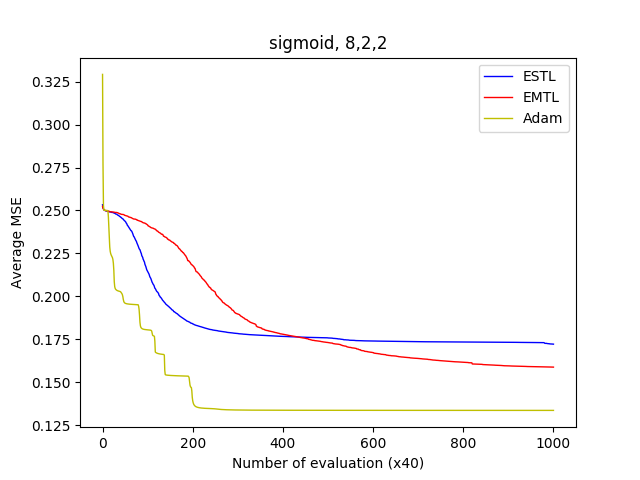
\includegraphics[width=1.0\linewidth]{images/sigmoid/avg_mse8,2,2.png}
      \end{subfigure}
      \begin{subfigure}{0.48\linewidth}
        \centering
        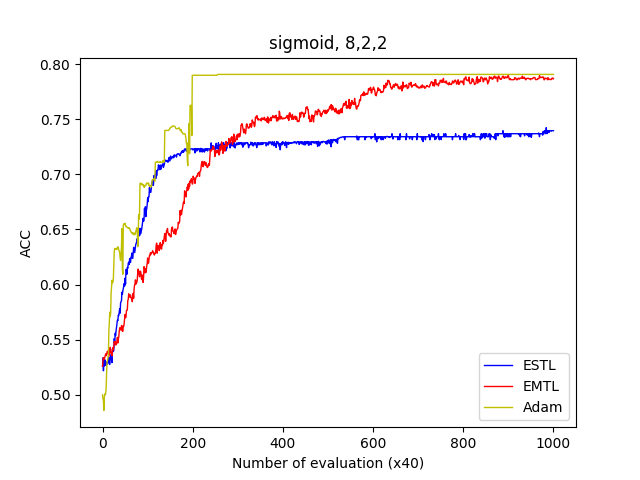
\includegraphics[width=1.0\linewidth]{images/sigmoid/avg_acc8,2,2.png}
      \end{subfigure}

      \begin{subfigure}{0.48\linewidth}
        \centering
        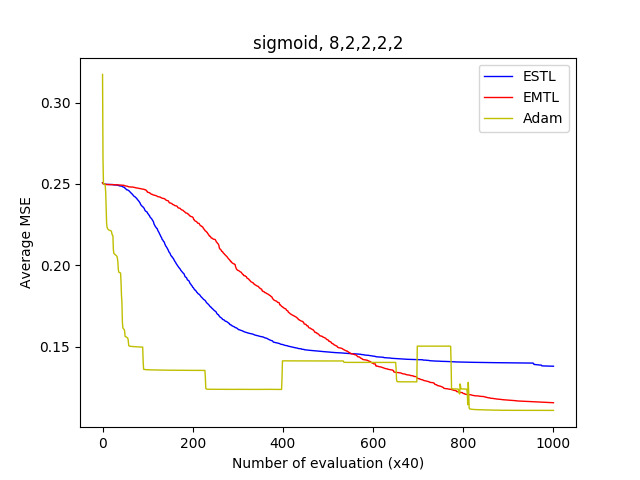
\includegraphics[width=1.0\linewidth]{images/sigmoid/avg_mse8,2,2,2,2.png}
      \end{subfigure}
      \begin{subfigure}{0.48\linewidth}
        \centering
        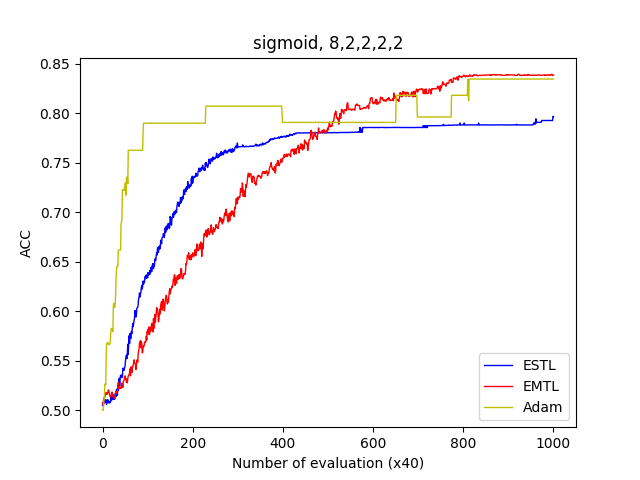
\includegraphics[width=1.0\linewidth]{images/sigmoid/avg_acc8,2,2,2,2.png}
      \end{subfigure}

      \begin{subfigure}{0.48\linewidth}
        \centering
        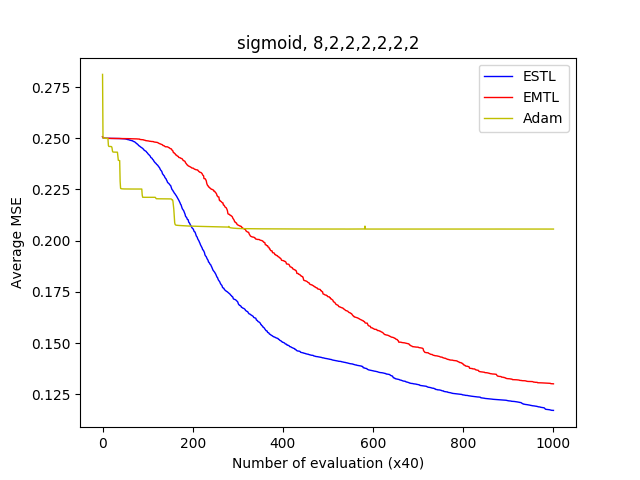
\includegraphics[width=1.0\linewidth]{images/sigmoid/avg_mse8,2,2,2,2,2,2.png}
      \end{subfigure}
      \begin{subfigure}{0.48\linewidth}
        \centering
        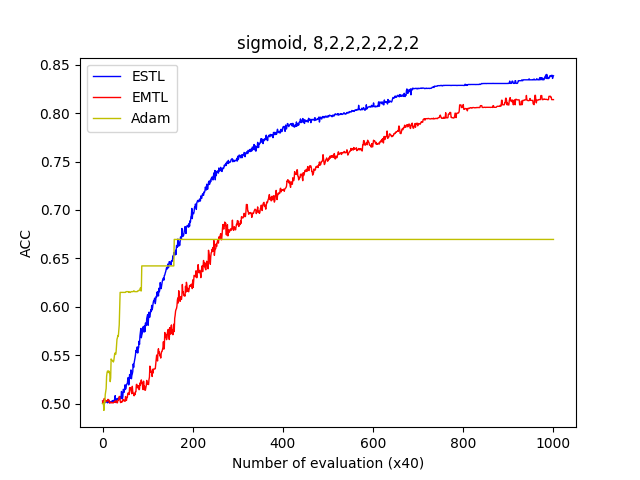
\includegraphics[width=1.0\linewidth]{images/sigmoid/avg_acc8,2,2,2,2,2,2.png}
      \end{subfigure}

      \caption{MSE and ACC results for networks using sigmoid activation for hidden units}
    \end{figure*}

  \subsection{Hidden unit with tanh activation}
    \begin{figure*}
      \centering
      \begin{subfigure}{0.48\linewidth}
        \centering
        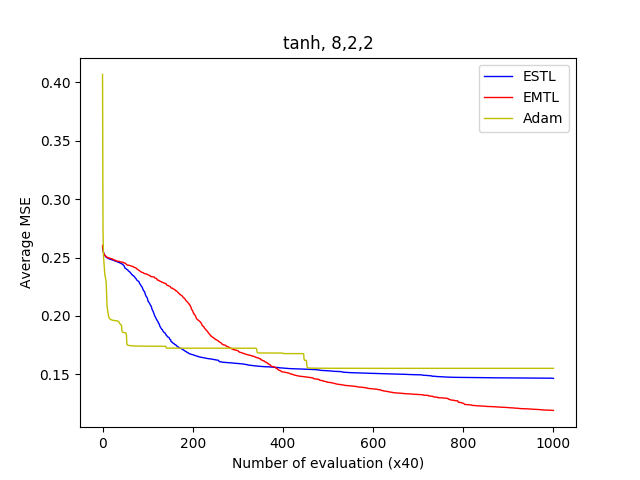
\includegraphics[width=1.0\linewidth]{images/tanh/avg_mse8,2,2.png}
      \end{subfigure}
      \begin{subfigure}{0.48\linewidth}
        \centering
        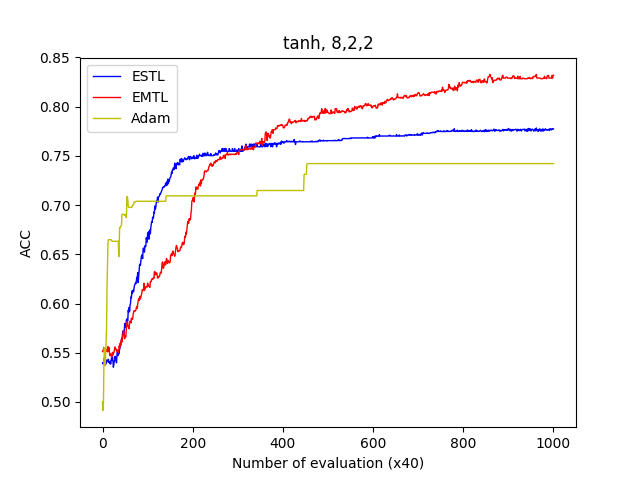
\includegraphics[width=1.0\linewidth]{images/tanh/avg_acc8,2,2.png}
      \end{subfigure}

      \begin{subfigure}{0.48\linewidth}
        \centering
        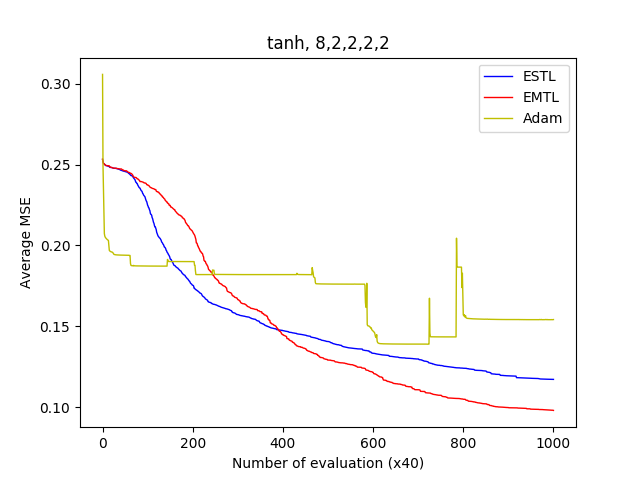
\includegraphics[width=1.0\linewidth]{images/tanh/avg_mse8,2,2,2,2.png}
      \end{subfigure}
      \begin{subfigure}{0.48\linewidth}
        \centering
        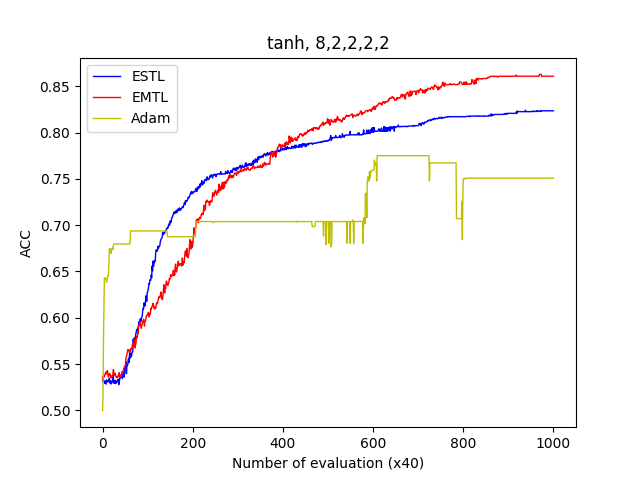
\includegraphics[width=1.0\linewidth]{images/tanh/avg_acc8,2,2,2,2.png}
      \end{subfigure}

      \begin{subfigure}{0.48\linewidth}
        \centering
        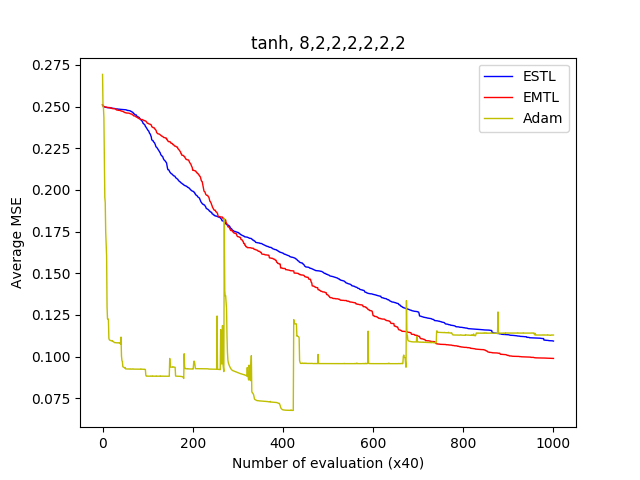
\includegraphics[width=1.0\linewidth]{images/tanh/avg_mse8,2,2,2,2,2,2.png}
      \end{subfigure}
      \begin{subfigure}{0.48\linewidth}
        \centering
        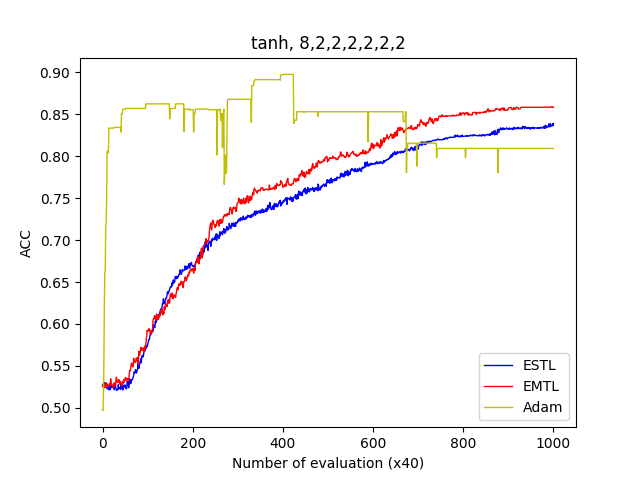
\includegraphics[width=1.0\linewidth]{images/tanh/avg_acc8,2,2,2,2,2,2.png}
      \end{subfigure}
    \end{figure*}

  \subsection{Hidden unit with relu activation}
    \begin{figure*}
      \centering
      \begin{subfigure}{0.48\linewidth}
        \centering
        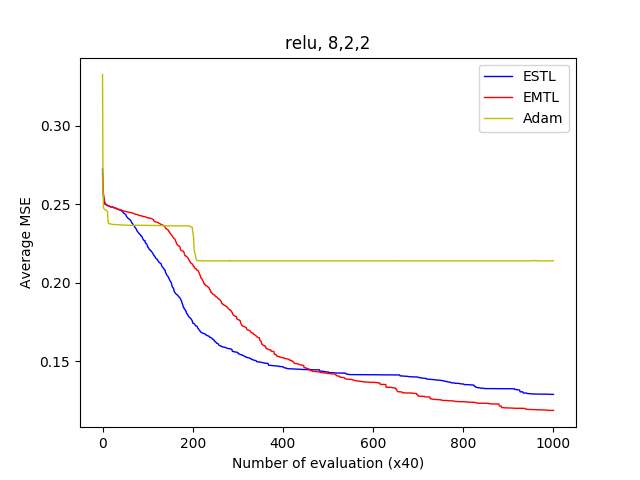
\includegraphics[width=1.0\linewidth]{images/relu/avg_mse8,2,2.png}
      \end{subfigure}
      \begin{subfigure}{0.48\linewidth}
        \centering
        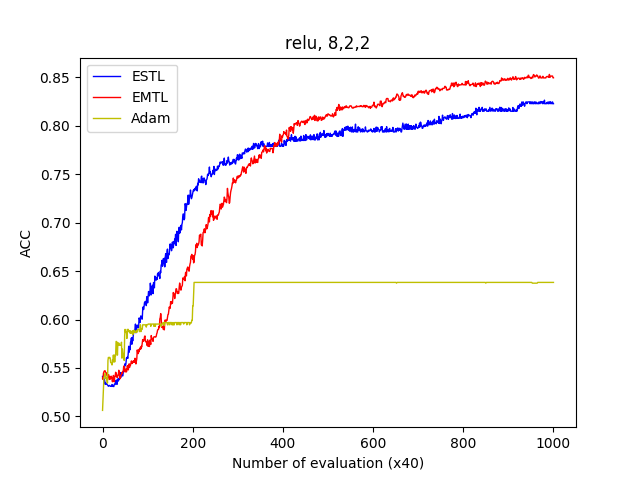
\includegraphics[width=1.0\linewidth]{images/relu/avg_acc8,2,2.png}
      \end{subfigure}

      \begin{subfigure}{0.48\linewidth}
        \centering
        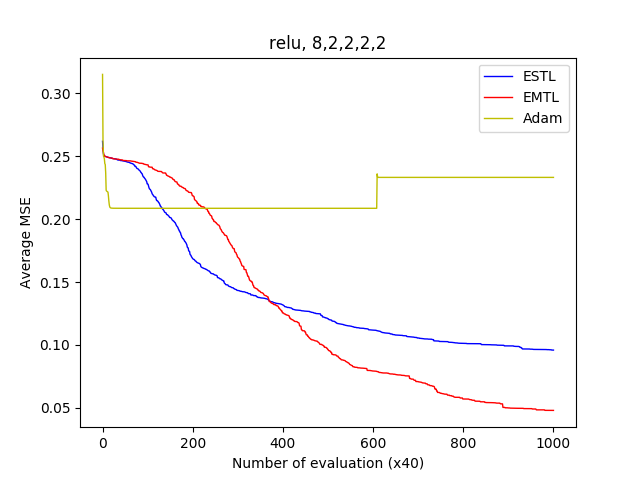
\includegraphics[width=1.0\linewidth]{images/relu/avg_mse8,2,2,2,2.png}
      \end{subfigure}
      \begin{subfigure}{0.48\linewidth}
        \centering
        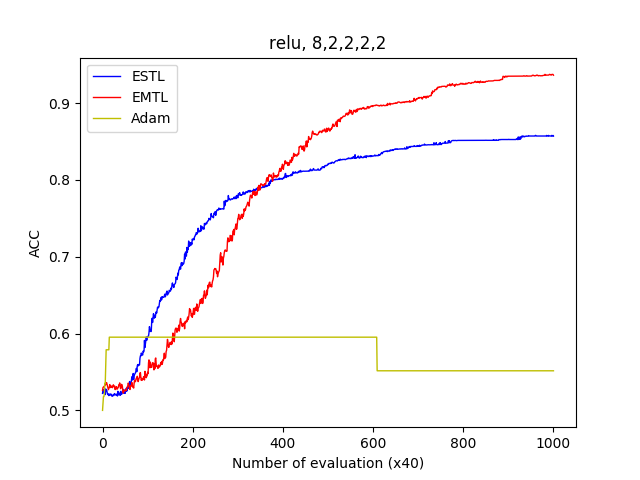
\includegraphics[width=1.0\linewidth]{images/relu/avg_acc8,2,2,2,2.png}
      \end{subfigure}

      \begin{subfigure}{0.48\linewidth}
        \centering
        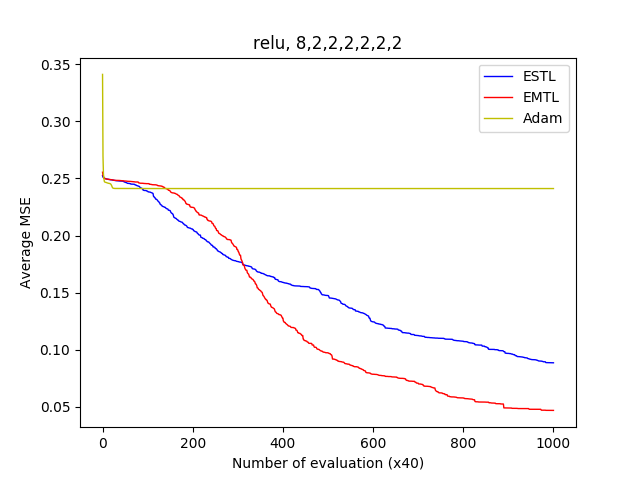
\includegraphics[width=1.0\linewidth]{images/relu/avg_mse8,2,2,2,2,2,2.png}
      \end{subfigure}
      \begin{subfigure}{0.48\linewidth}
        \centering
        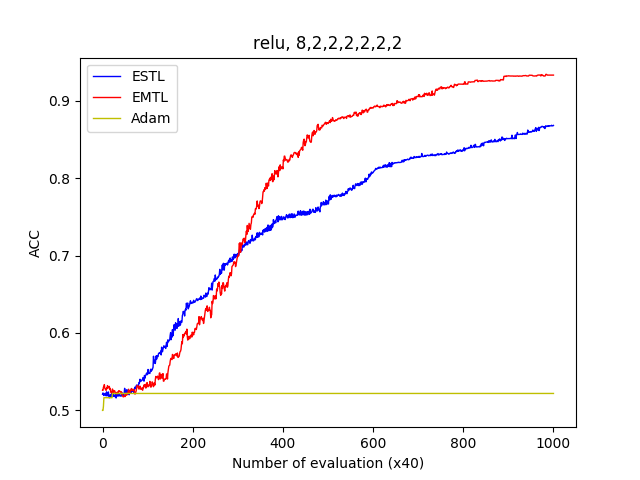
\includegraphics[width=1.0\linewidth]{images/relu/avg_acc8,2,2,2,2,2,2.png}
      \end{subfigure}
    \end{figure*}

\section{Acknowledges}
  \cite{mfea-ffnn} \cite{mfea}

\printbibliography

\end{document}


